%!TEX TS-program = xelatex
\documentclass[12pt, a4paper, oneside]{article}

\usepackage{amsmath,amsfonts,amssymb,amsthm,mathtools}  % пакеты для математики

\usepackage[english, russian]{babel} % выбор языка для документа
\usepackage[utf8]{inputenc} % задание utf8 кодировки исходного tex файла
\usepackage[X2,T2A]{fontenc}        % кодировка

\usepackage{fontspec}         % пакет для подгрузки шрифтов
\setmainfont{Linux Libertine O}   % задаёт основной шрифт документа

\usepackage{unicode-math}     % пакет для установки математического шрифта
\setmathfont[math-style=upright]{Neo Euler} % шрифт для математики


%%%%%%%%%% Работа с картинками %%%%%%%%%
\usepackage{graphicx}                  % Для вставки рисунков
\usepackage{graphics}
\graphicspath{{images/}{pictures/}}    % можно указать папки с картинками
\usepackage{wrapfig}                   % Обтекание рисунков и таблиц текстом

%%%%%%%%%%%%%%%%%%%%%%%% Графики и рисование %%%%%%%%%%%%%%%%%%%%%%%%%%%%%%%%%
\usepackage{tikz, pgfplots}  % язык для рисования графики из latex'a

%%%%%%%%%% Гиперссылки %%%%%%%%%%
\usepackage{xcolor}              % разные цвета

\usepackage{hyperref}
\hypersetup{
	unicode=true,           % позволяет использовать юникодные символы
	colorlinks=true,       	% true - цветные ссылки, false - ссылки в рамках
	urlcolor=blue,          % цвет ссылки на url
	linkcolor=red,          % внутренние ссылки
	citecolor=green,        % на библиографию
	pdfnewwindow=true,      % при щелчке в pdf на ссылку откроется новый pdf
	breaklinks              % если ссылка не умещается в одну строку, разбивать ли ее на две части?
}


\usepackage{todonotes} % для вставки в документ заметок о том, что осталось сделать
% \todo{Здесь надо коэффициенты исправить}
% \missingfigure{Здесь будет Последний день Помпеи}
% \listoftodos --- печатает все поставленные \todo'шки

\usepackage[paper=a4paper, top=20mm, bottom=15mm,left=20mm,right=15mm]{geometry}
\usepackage{indentfirst}       % установка отступа в первом абзаце главы

\usepackage{setspace}
\setstretch{1.15}  % Межстрочный интервал
\setlength{\parskip}{4mm}   % Расстояние между абзацами
% Разные длины в латехе https://en.wikibooks.org/wiki/LaTeX/Lengths


\usepackage{xcolor} % Enabling mixing colors and color's call by 'svgnames'

\definecolor{MyColor1}{rgb}{0.2,0.4,0.6} %mix personal color
\newcommand{\textb}{\color{Black} \usefont{OT1}{lmss}{m}{n}}
\newcommand{\blue}{\color{MyColor1} \usefont{OT1}{lmss}{m}{n}}
\newcommand{\blueb}{\color{MyColor1} \usefont{OT1}{lmss}{b}{n}}
\newcommand{\red}{\color{LightCoral} \usefont{OT1}{lmss}{m}{n}}
\newcommand{\green}{\color{Turquoise} \usefont{OT1}{lmss}{m}{n}}

\usepackage{titlesec}
\usepackage{sectsty}
%%%%%%%%%%%%%%%%%%%%%%%%
%set section/subsections HEADINGS font and color
\sectionfont{\color{MyColor1}}  % sets colour of sections
\subsectionfont{\color{MyColor1}}  % sets colour of sections

%set section enumerator to arabic number (see footnotes markings alternatives)
\renewcommand\thesection{\arabic{section}.} %define sections numbering
\renewcommand\thesubsection{\thesection\arabic{subsection}} %subsec.num.

%define new section style
\newcommand{\mysection}{
	\titleformat{\section} [runin] {\usefont{OT1}{lmss}{b}{n}\color{MyColor1}} 
	{\thesection} {3pt} {} } 


%	CAPTIONS
\usepackage{caption}
\usepackage{subcaption}
%%%%%%%%%%%%%%%%%%%%%%%%
\captionsetup[figure]{labelfont={color=Turquoise}}

\pagestyle{empty}


%%%%%%%%%% Свои команды %%%%%%%%%%
\usepackage{etoolbox}    % логические операторы для своих макросов

% Все свои команды лучше всего определять не по ходу текста, как это сделано в этом документе, а в преамбуле!

% Одно из применений - уничтожение какого-то куска текста!
\newbool{answers}
\booltrue{answers}
%\boolfalse{answers}

\newbool{addanswers}
\booltrue{addanswers}
%\boolfalse{addanswers}

\usepackage{enumitem}
% бульпоинты в списках
\definecolor{myblue}{rgb}{0, 0.45, 0.70}
\newcommand*{\MyPoint}{\tikz \draw [baseline, fill=myblue,draw=blue] circle (2.5pt);}
\renewcommand{\labelitemi}{\MyPoint}

% расстояние в списках
\setlist[itemize]{parsep=0.4em,itemsep=0em,topsep=0ex}
\setlist[enumerate]{parsep=0.4em,itemsep=0em,topsep=0ex}

\begin{document}

\section*{Семинар 8-9:  сегментация клиентов и кластеризация}

\subsection*{Задача 1 }

\begin{enumerate}

\item[а)] У нас есть точки $A(1,1)$, $B(2,2)$, $C(3,0)$. Нарисуйте их на плоскости и посчитайте между ними расстояние Евклида, Манхеттенское и Чебышева: 

\begin{equation}
\begin{aligned}
& \rho_1(A,B) = \sqrt{(x_B - x_A)^2 + (y_B - y_A)^2} \\ 
& \rho_2(A,B) = |x_B - x_A| + |y_B - y_A|  \\
& \rho_3(A,B) = \max(|x_B - x_A|, |y_B - y_A|) \\
\end{aligned}
\end{equation}


\item[б)] Какое расстояние будете использовать для того, чтобы добраться из точки А в точку Б? Почему? 

\begin{minipage}[t]{0.45\textwidth}
	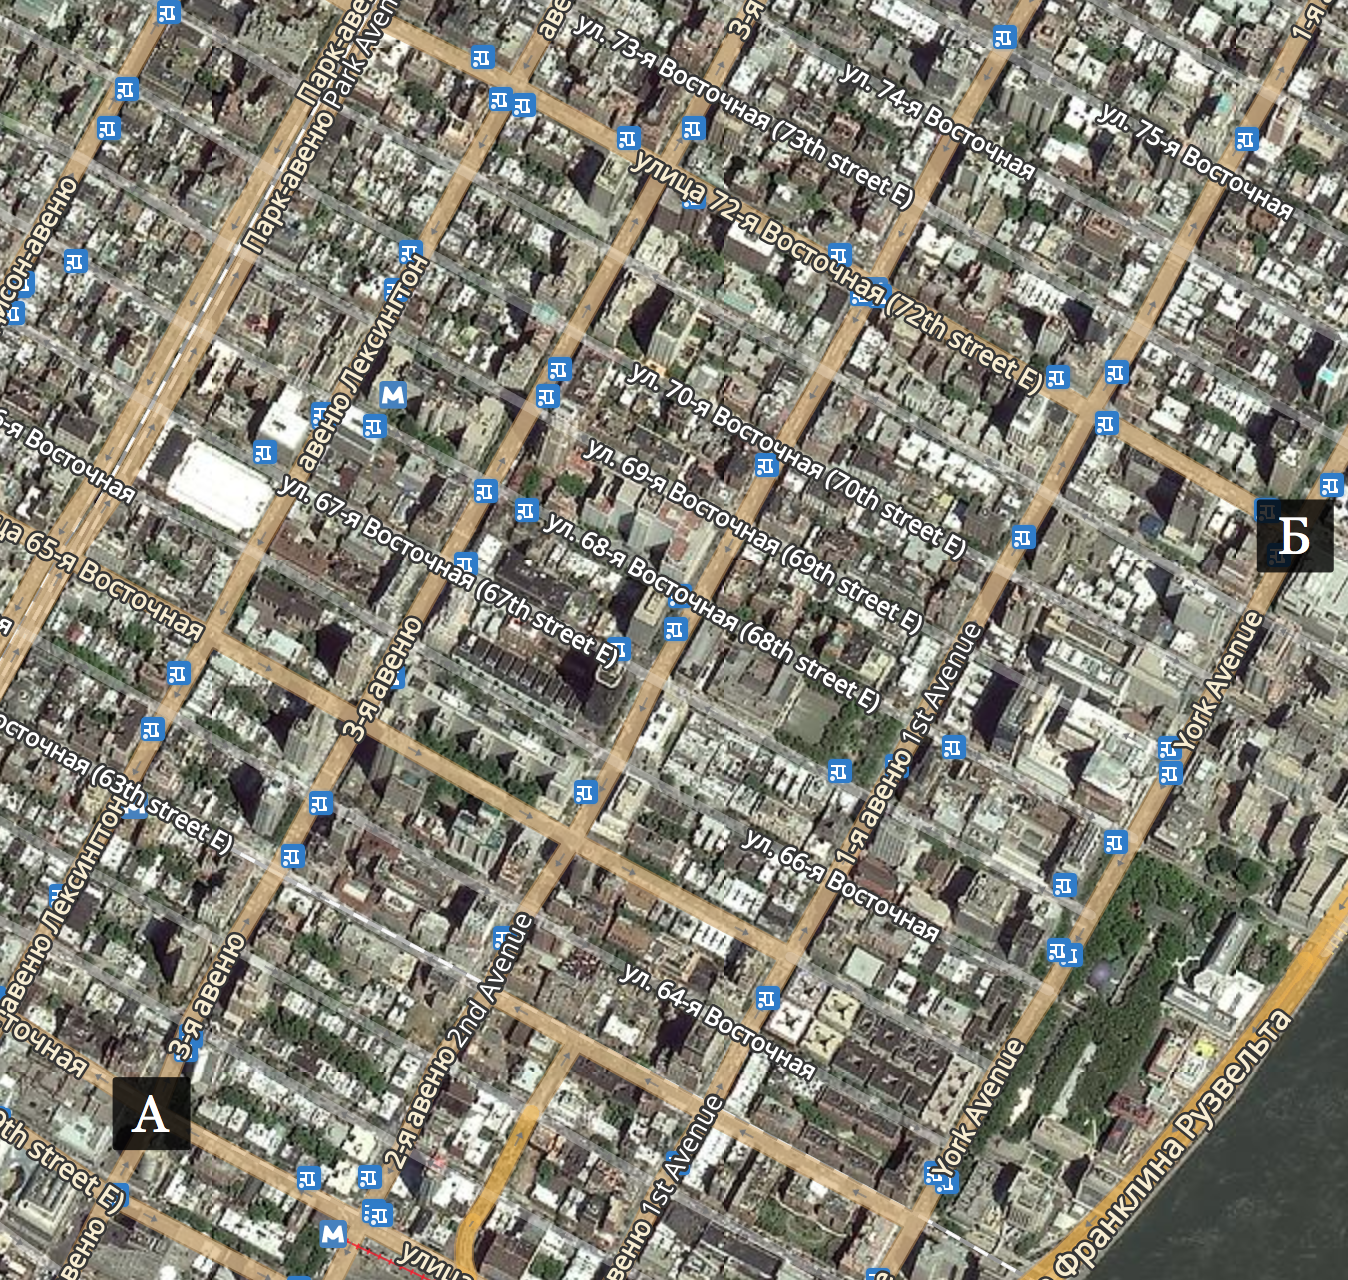
\includegraphics[scale=0.12]{metr_1.png}
\end{minipage}
\hfill
\begin{minipage}[t]{0.45\textwidth}
	\includegraphics[scale=0.12]{metr_2.png}
\end{minipage}

\item[в)] Какое расстояние вы бы использовали для измерения похожести текстов или генома?

\begin{center}
	\includegraphics[scale=0.3]{metr_3.png}
\end{center}

\end{enumerate}

\ifbool{answers}{
	\textbf{Решение:}
	
Начнём с расстояний. Для примера посчитаем все три между точками $A$ и $B$: 

\begin{equation}
\begin{aligned}
& \rho_1(A,B) = \sqrt{(2-1)^2 + (2 - 1)^2}  = \sqrt{2} \\ 
& \rho_2(A,B) = |2-1| + |2-1| = 1 + 1 = 2  \\
& \rho_3(A,B) = \max(|2-1|, |2-1|) = \max(1,1) = 1 \\
\end{aligned}
\end{equation}
	
	
По аналогии посчитаем все расстояния и выпишем результаты в табличку: 
	
	\begin{center}
		\begin{tabular}{c|c|c|c}
			\hline
			 & Евклидово & Манхеттенское & Чебышева \\
			\hline
			$AB$  & $\sqrt{2}$ & $2$ &   $1$ \\
			$AC$  & $\sqrt{5}$ & $3$ &   $2$ \\
			$BC$  & $\sqrt{5}$ & $3$ &   $2$ \\
		\end{tabular}
	\end{center}
	
Изобразим все три ситуации на декартовой плоскости.  В каждой ситуации растояния считаются <<по пунктиру>>. Для расстояния Евклида по диагонали, для Манхеттенского растояния сначала по одной оси, затем по другой, для расстояния Чебышёва берётся только одна координата - та, по которой дольше всего идти. 

\begin{center}
	\includegraphics[scale=0.25]{distantions.png}
\end{center}	

Для случая а) мы находимся в городе. Мы не можем идти напролом через здания, нам приходится идти по улицам. Логичным будет использовать манхеттенское расстояние. Обратите внимание, что оно обладает интересным свойством: неважно где сворачивать. Идя ко красной дороге, мы пройдём ровно столько же, если бы пошли по синей. 

В случае б) можно использовать расстояние Евклида, так как мы идём по полю да по лесу. 
	
\begin{minipage}[t]{0.45\textwidth}
	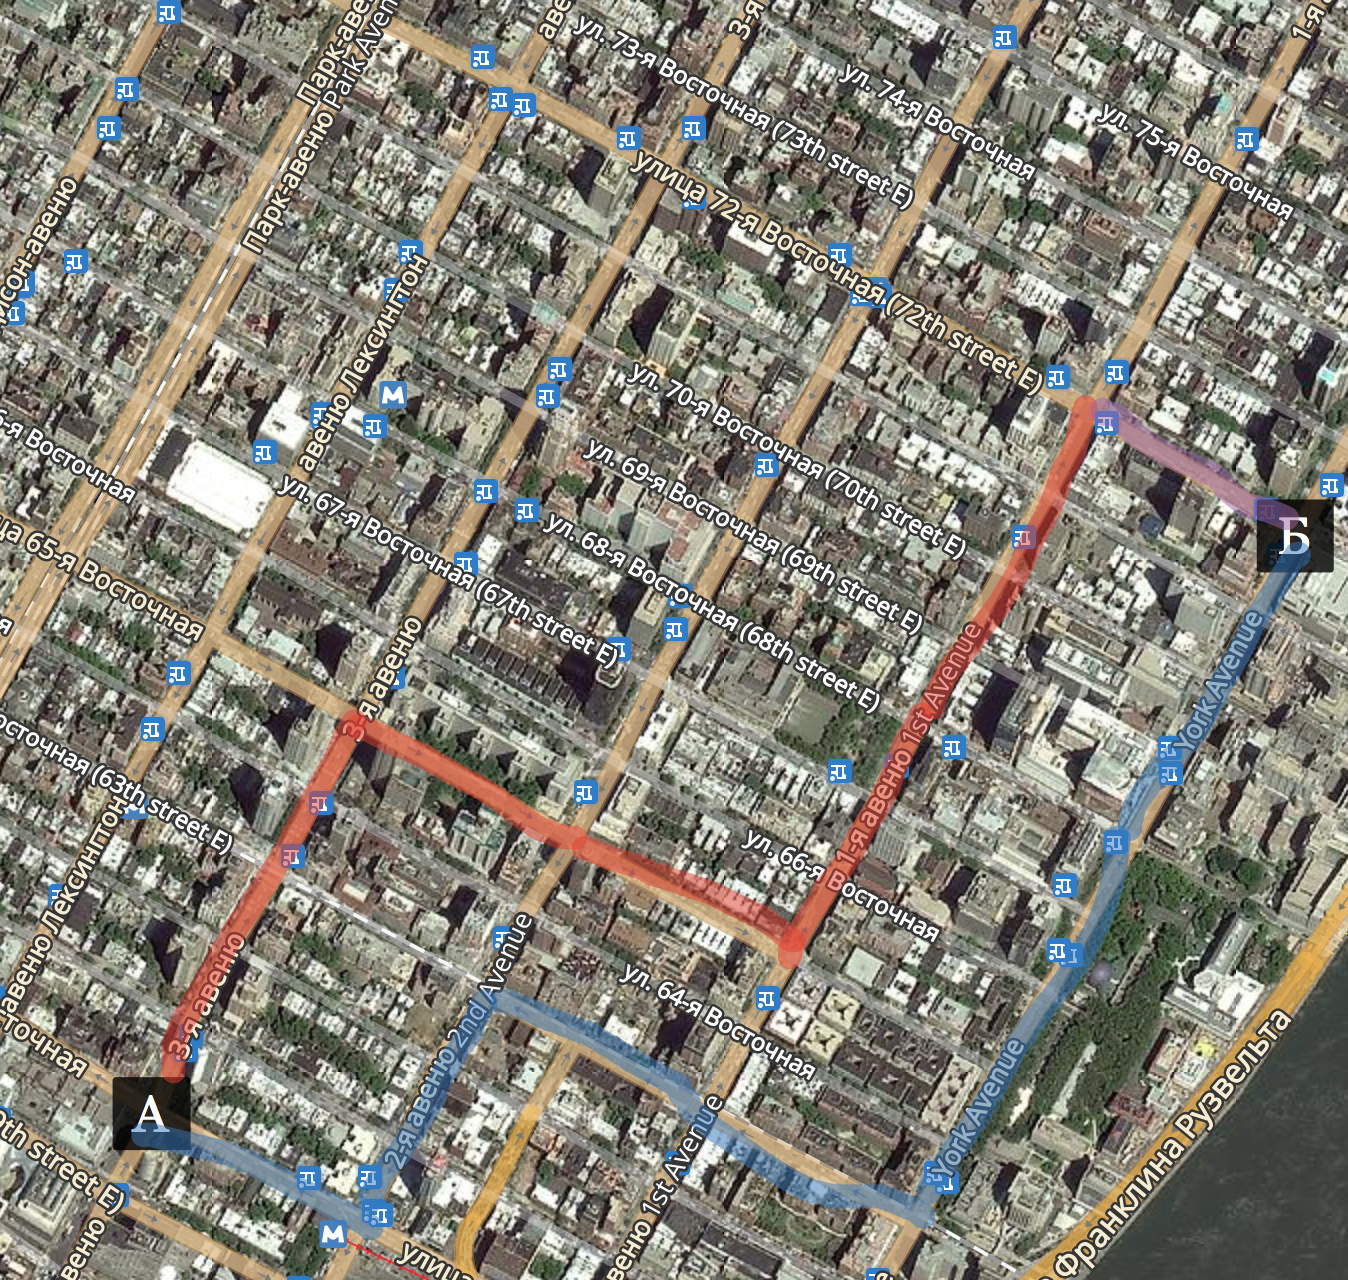
\includegraphics[scale=0.12]{metr_1_ans.png}
\end{minipage}
\hfill
\begin{minipage}[t]{0.45\textwidth}
	\includegraphics[scale=0.12]{metr_2_ans.png}
\end{minipage}
	
Для того, того, чтобы понять насколько похожи тексты, можно использовать расстояние Левенштейна.  Это минимальное количество операций вставки одного символа, удаления одного символа и замены одного символа на другой, необходимых для превращения одной строки в другую. 

Ровно его же можно использовать для последовательностей нуклеотидов. В нашем случае зелёным показано сколько надо нуклеотидов заменить, а красным сколько надо вставить. Расстояние левенштейна между представленными в примере текстами: $2$ (буквы о и ч). Между последовательностями: $14$.
}


\subsection*{Задача 2}

Жокей Святополк решил открыть несколько новых ларьков с шаурмой\footnote{По мотивам \url{https://vas3k.ru/blog/machine_learning/}}. Перед открытием он подумал о потенциальных покупателях и выяснил, где на районе находятся общежития.  На картинках ниже они отмечены синими точками.  Святополк понимает, что все общежития, расположенные в районе, можно сегментировать по их географическому положению и, исходя из этого, расположить палатки с шаурмой. Сделать  это ему хотелось бы с помощью алгоритма $K-means$:

\begin{enumerate}
	\item Ставим ларьки с шаурмой в случайных местах;
	\item Смотрим в какой кому ближе идти;
	\item Двигаем ларьки ближе к центрам их популярности;
	\item Снова смотрим и двигаем;
	\item Повторяем так много раз, пока алгоритм не сойдётся и движение не прекратится.
\end{enumerate}

\begin{minipage}[t]{0.45\textwidth}
\includegraphics[scale=0.5]{knn1.png}
\end{minipage}
\hfill
\begin{minipage}[t]{0.45\textwidth}
\includegraphics[scale=0.5]{knn2.png}
\end{minipage}

Красными точками отмечены стартовые точки для палаток. В первом районе Святополк ставит две палатки, во втором районе три палатки.  Помогите Святополку с сегментацией! Сколько итераций понадобилось сделать до полной сходимости алгоритма? Сколько объектов вошли в каждый из кластеров?  

\begin{enumerate}
	\item[а)] Используйте для кластеризации Евклидово расстояние.
	\item[б)] Используйте для кластеризации Манхеттенское расстояние.
	\item[в)] В этой задачке мы сами предложили вам для кластеризации начальные точки (красные квадраты). На практике начальное приближение центроидов обычно генерирует компьютер.  Изменится ли разбиение на кластеры, если изменить стартовые точки?
\end{enumerate}

\ifbool{answers}{
	\textbf{Решение:}

\begin{enumerate}
	\item[а)]  Первый случай элементарный. Все растояния видны на глазок. Даже ничего считать не надо. В ходе первой итерации сразу понятно, что все левые точки отходят второму кластеру и только одна первому.  Центр первого кластера переезжает в своего единственного последователя. Центр второго кластера найдём как средневзвешенное координат его последователей: 
	
	\begin{equation}
	\begin{aligned}
&	x_2 = \frac{1}{4} \cdot (-3 -2 -1 + 1) = - \frac{5}{4} \\ 
&	y_2 = \frac{1}{4} \cdot (0 + 0 + 0 + 0) = 0 \\ 
	\end{aligned}
	\end{equation}
	
	\begin{minipage}[t]{0.45\textwidth}
		\includegraphics[scale=0.25]{k_means_a1.png}
	\end{minipage}
	\hfill
	\begin{minipage}[t]{0.45\textwidth}
		\includegraphics[scale=0.25]{k_means_a2.png}
	\end{minipage}

На второй итерации последователи появляются у обоих ларьков. Первый центр оказывается ровно между своими двумя последователями в точке $(0,1.5)$. Второй центр пересчитаем как средневзвешеной троих последователей: 

\begin{equation}
\begin{aligned}
& x_2 = \frac{1}{3} \cdot (-3 -2 -1 ) = - 2 \\ 
& y_2 = \frac{1}{3} \cdot (0 + 0 + 0 ) = 0 \\ 
\end{aligned}
\end{equation}


\begin{center}
	\includegraphics[scale=0.25]{k_means_a3.png}
\end{center}

После второй итерации центры больше не обмениваются последователями. Это означает, что алгоритм сошёлся и мы нашли оптимальные точки для ларьков. Первый находится между двумя правыми общагами, второй в одной из левых общаг. Кому-то повезло.  

Проделаем всё то же самое со второй ситуацией.  На первом шаге второй и третий ларёк переезжают в конкретные общаги. Для первого ларька по-честному нужно посчитать координаты нового центра: 

\begin{equation}
\begin{aligned}
& x_1 = \frac{1}{5} \cdot (0 + 0 -2 -3 -3) = - \frac{8}{5} \\ 
& y_1 = \frac{1}{5} \cdot (1 - 1 + 0 + 0 + 0 ) = 0 \\ 
\end{aligned}
\end{equation}
	

\begin{minipage}[t]{0.45\textwidth}
\includegraphics[scale=0.25]{k_means_b1.png}
\end{minipage}
\hfill
\begin{minipage}[t]{0.45\textwidth}
	\includegraphics[scale=0.25]{k_means_b2.png}
\end{minipage}

На второй итерации часть последователей перебегает от первого ларька ко второму. Для третьего ларька ничего не меняется. Снова пересчитываем координаты новых центров: 

\begin{equation}
\begin{aligned}
& x_1 = \frac{1}{3} \cdot (-2 -3 -3) = - \frac{8}{3} \\ 
& y_1 = \frac{1}{3} \cdot (0 + 0 - 1 ) = -\frac{1}{3} \\ 
& x_2 = \frac{1}{3} \cdot (0 + 0 + 1) =  \frac{1}{3} \\ 
& y_2 = \frac{1}{3} \cdot (0 + 0 + 1) =  \frac{1}{3} \\ 
\end{aligned}
\end{equation}

\begin{minipage}[t]{0.45\textwidth}
	\includegraphics[scale=0.25]{k_means_b3.png}
\end{minipage}
\hfill
\begin{minipage}[t]{0.45\textwidth}
	\includegraphics[scale=0.25]{k_means_b4.png}
\end{minipage}

После второй итерации вроде как всё стабилизируется. Есть только одна подозрительная точка, отмеченная на рисунке надписью, которую сложно не заметить. Давайте по-честному посчитаем расстояние от неё до  центров второго и третьего кластеров: 

\begin{equation}
\begin{aligned}
& \rho_3 = \sqrt{(1 - 2)^2 + (0 - 0)^2} = 1 \\ 
& \rho_2 = \sqrt{(1 - 1/3)^2 + (0 - 1/3)^2} \approx 0.74 \\ 
\end{aligned}
\end{equation}

Оказывается, что она ближе ко второму ларьку. На этом, после двух итераций алгоритм прекращает работу. 

	\item[б)]  В первой ситуации результат будет ровно таким же. Мы с какого-то момента начинаем считать расстояния только по оси $x$. Из-за этого результат выходит одинаковым. 

	Во второй ситуации первые две итерации будут ровно такими же. В самом конце неожиданно окажется, что спорная точка действительно является спорной. 
	
	\begin{equation}
	\begin{aligned}
	& \rho_3 = |1 - 2| + | 0 - 0| = 1\\ 
	& \rho_2 = |1 - 1/3|  + | 0 - 1/3| = 1 \\ 
	\end{aligned}
	\end{equation}
	
Не очень понятно, к какому кластеру её отнести. Можно либо остановить на этом алгоритм, либо сделать ещё один шаг и тогда кластеры окончательно зафиксируются. 
	
\begin{center}
	\includegraphics[scale=0.25]{k_means_b5.png}
\end{center}
	
	 
	\item[в)]  В первом случае нет. Кластеры выделены очень хорошо. Во втором случае да. Если взять в качестве начальных точек $(0,-1)$, $(0,2.1)$, $(3,0)$, то в ходе Евклидового $k-means$ мы придём к такой же ситуации, как в случае Манхеттенской метрики в конце прошлого пункта.
\end{enumerate}
}


\subsection*{Задача 3 }

Начальник Аристарх был в командировке. Там он услышал про иерархическую агломеративную кластеризацию. По приезду, находясь в состоянии восторга, он записал в свой блокнот следующие четыре наблюдения:

\begin{center}
\begin{tabular}{c|c|c}
	\hline
	$n$  & $x$ & $z$ \\
	\hline
	1 & 8 & 6   \\
	2 & 6 & 10 \\
	3 & 2 & 4   \\
	4 & 4 & 2   \\
\end{tabular}
\end{center}

После он отдал блокнот маркетологу Савелию. Аристарх хочет, чтобы Савелий провел агломеративную иерархическую кластеризацию.  На совещаний было решено использовать в качестве расстояния между объектами обычное Евклидово расстояние. Расстояние между кластерами решено определять по принципу дальнего соседа. Помогите Савелию с агломеративной иерархической кластеризацией. И не забудьте нарисовать дендрограмму. Начальники любят красивые картинки. 

\ifbool{answers}{
	\textbf{Решение:}
	
	Вспомним алгоритм агломерационной иерархической кластеризации:
	
	\begin{enumerate}
		\item  Начинаем с того, что высыпаем на каждую точку свой кластер
		\item  Сортируем попарные расстояния между центрами кластеров по возрастанию
		\item  Берём пару ближайших кластеров, склеиваем их в один и пересчитываем центр кластера
		\item  Повторяем п. 2 и 3 до тех пор, пока все данные не склеятся в один кластер
	\end{enumerate}

Для удобства сразу же посчитаем расстояния между всеми точками и занесём его в табличку:

\begin{center}
	\begin{tabular}{c|c}
		$12$ & $\sqrt{20}$   \\
		\hline
		$13$ & $\sqrt{40}$ \\
		\hline
		$14$ & $\sqrt{32}$   \\
		\hline
		$23$ & $\sqrt{52}$  \\
		\hline
		$24$ & $\sqrt{68}$   \\
		\hline
		$34$ & $\sqrt{8}$  \\
	\end{tabular}
\end{center}

На первой итерации каждое наблюдение это отдельный кластер.  Самое короткое расстояние между $3$ и $4$ наблюдениями. Сольём их в единый кластер. 

\begin{minipage}[t]{0.45\textwidth}
	\includegraphics[scale=0.25]{ekl1.png}
\end{minipage}
\hfill
\begin{minipage}[t]{0.45\textwidth}
	\includegraphics[scale=0.25]{ekl2.png}
\end{minipage}


Кластера $IV$ больше нет. Теперь нам надо посчитать расстояние между оставшимися кластерами. Расстояние от $I$ до $II$ соотвествует $\sqrt{20}$, как и раньше. Расстояние от $III$ до $I$ надо выбрать по принципу дальнего соседа. Третье наблюдение дальше от первого, чем четвёртое. Выходит, что расстояние между $III$ и $I$ равно $\sqrt{40}$. Четвёртое наблюдение дальше от второго, чем третье. Расстояние между $III$ и $II$ равно $\sqrt{68}$. Сливаем между собой кластеры $I$ и $II$. 

В игре остаются кластеры $I$ и $III$.  Давайте выясним какое между ними расстояние. Оно, по-прежнему, формируется по принципу дальнего соседа. Среди четырёх расстояний: $13, 14, 23, 24$ нам нужно выбрать самое большое. Это расстояние от второй точки до четвёртой, $\sqrt{68}$.


\begin{minipage}[t]{0.45\textwidth}
	\includegraphics[scale=0.25]{ekl3.png}
\end{minipage}
\hfill
\begin{minipage}[t]{0.45\textwidth}
	\includegraphics[scale=0.2]{ekl4.png}
\end{minipage}

Теперь мы можем построить дендрограмму. Сначала соединились $3$ и $4$  наблюдения, расстояние между нии составило $\sqrt{8}$. После $1$ и $2$ с расстоянием между ними $\sqrt{20}$. После слились два кластера с расстоянием между ними $\sqrt{68}$. На дендрограмме длина линии до точки слияния соответствует расстоянию между кластерами. 
}



\subsection*{Задача 4} 

Маркетолог с аналитическим складом ума Оля (она кстати говоря ещё и фрилансер) занимается заказом от туристической фирмы. Ей нужно сделать с помощью методов машинного обучения сегментацию клиентов. На этапе предобработки фичей Оля столкнулась с двумя проблемами: категориальной переменной $x$, в которой записаны курорты и текстовой переменной $z$, в которой дан отзыв о курорте:

\begin{center}
	\begin{tabular}{c|c|c}
		\hline
		$n$ & $x$ & $z$ \\
		\hline
		1 & Испания  & Нежился на пляже  \\
		2 & Крым  &  Копали яму на пляже\\
		3 & Дача  &  Копал картошку  \\
		4 & Крым  & Ел картошки и картошку \\
	\end{tabular}
\end{center}

\begin{enumerate} 
	\item[a)]  Что такое категориальная переменная? Почему её надо как-то предобрабатывать? 
	\item[б)]  Почему нельзя сделать замену Крым $=1$, Дача $=2$, Испания $=3$? Что такое OHE-кодирование? Как будет выглядеть наша табличка с переменными после OHE?
	\item[в)]  Почему нельзя сделать OHE для текстовой переменной?
	\item[г)]  Какие этапы предобработки тестов вы знаете? На самом деле вы их скорее всего не знаете и мы их сейчас обсудим. 
	\item[д)] Сделайте для корпуса текстов из задачки tf-idf. 
\end{enumerate}

\ifbool{answers}{
	\textbf{Решение:}

\begin{enumerate} 
\item[а)]  Категориальная переменная - это переменная, которая принимает значения из некоторого конечного множества. В данном случае переменная $x$ принимает значение из множества курортов. Модели обучаются на каких-то числовых данных. Наша категориальная переменная не числовая. Чтобы обучить модель, мы должны переработать её в числовой вид.

\item[б)]  Нельзя сделть замену Крым $=1$, Дача $=2$, Испания $=3$, потому что в таком случае модель подумает, что на множестве курортов есть отношение порядка, то есть, что Крым лучше Дачи, а Дача лучше Испании. Это далеко не так. Для каждого человека на множестве курортов свой субъективный порядок. Модель же должна быть объективной.  

Для того, чтобы нормально преобразовать курорты в цифры, обычно используют one hot encoding (одно горячее кодирование)00))0). 

Для каждой категории вводится своя дамми-переменная, принимающая значение $1$, если человек был на этом курорте и значение $0$, если не был. Наша табличка преображается. Одна катгориальная переменная превращается в несколько бинарных.

Обратите внимание, что полученая таблица избыточна.

\begin{center}
	\begin{tabular}{c|c|c|c}
		\hline
		$n$ & $x_{isp}$ & $x_{kr}$ & $x_{da}$\\
		\hline
		1 & 1  & 0 & 0   \\
		2 & 0  & 1 & 0  \\
		3 & 0 & 0  & 1  \\
		4 & 0 & 1 & 0  \\
	\end{tabular}
\end{center}

Легко можно избавиться от одной из переменных и не потерять при этом информацию. Если мы выбросим переменную $x_{da}$, мы увидем в оставшихся двух переменных нули, сразу же поймём, что человек был на даче. 

 Лучше выбросить одну избыточную переменную, иначе можно попасть в не очень хорошую ситуацию, которая называется \textbf{дамми-ловушкой.}  Предположим, что мы оцениваем модель линейной регресси: 

\[ y_i = \beta_0 + \beta_1 \cdot x_{isp} + beta_2 \cdot x_{kr} + \beta_3 \cdot x_{da}. \]

В такой ситуации мы нарываемся на линейную зависимость. Константа равна сумме дамми-переменных. Мы попадаем в ситуацию мультиколинеарности. Если мы будем учить модель без регуляризатора, у нас ничего не выйдет. 

\item[в)]  Потому что практически каждый текст уникален и наше OHE скорее всего приведёт к появлению $n-1$ дополнительной переменной. На будет недостаточно $n$ наблюдений, чтобы оценить адекватную модель. Приходится искать более изящные пути работы с текстами. 

\item[г)] Для текстов существует несколько этапов предобработки. Обычно это токенизация, нормализация (стемминг или лемматизация), очистка от стоп-слов. Подробнее об этом написано в юпитерском блокноте для текущего семинара.

\item[д)]  Разобьём все тексты на слова, очистим их от стоп-слов и нормальзуем. После, если в наблюдении встречается данное слово, будем ставить в табличке количество упоминаний, а если нет $0$.

\begin{center}
	\begin{tabular}{c|c|c|c|c|c|c}
		\hline
		 &нежиться & пляж & копать & яма & картошка & есть \\
		\hline
		1 &  1 & 1 & 0 & 0 & 0 & 0 \\
		2 & 0 & 1 & 1 & 1 & 0 & 0 \\
		3 & 0 & 0 & 1 & 0 & 1& 0 \\
		4 & 0 & 0 & 0 & 0 & 2 & 1 \\
	\end{tabular}
\end{center}

При достаточно большом числе текстов в корпусе, такую табличку можно использовать для обучения. Однако можно построить чуть более умные переменные. Для этого используется подход tf-idf. Предпосылки подхода:

\begin{itemize}
	\item Порядок слов неважен.
	\item Если слово встречается в документе часто и оно не является стоп-словом, скорее всего, оно важное. Эту тенденцию отражает показатель tf (сокращение от английского term frequency, частота слова). Чтобы получить tf, нам просто нужно нормализовать матрицу,  полученную выше на размер словаря.
	\item Если слово встречается в других документах реже, чем в данном, то, скорее всего, оно также важное, так как описывает специфику документа и отличает его от других. Эту тенденцию отражает показатель idf (сокращение от inverse document frequency, обратная частота документа). Обычно idf расчитывают как:
	
	\[ \ln \left( \frac{N}{n_i} \right), \]
	
	где $N$ --- объём словаря, $n_i$ --- количество документов, в которых встретилось слово $i$.
\end{itemize}

Логарифм берётся, чтобы сгладить очень большие числа. Перемножив tf и idf мы учтём оба факта важности слова и получим tf-idf представление текста. 

Построим матрицу для $tf$. В этом случае нормализация идёт по строкам:

\begin{center}
	\begin{tabular}{c|c|c|c|c|c|c}
		\hline
		&нежиться & пляж & копать & яма & картошка & есть \\
		\hline
		$1 $&  $1/6$ & $1/6$ & $0$ & $0 $& $0 $& $0$ \\
		$2$ & $0$ & $1/6$ & $1/6$ & $1/6$ & $0$ & $0$ \\
		$3$ & $0$ & $0$ & $1/6$ & $0$ & $1/6$ & $0$ \\
		$4$ &$ 0$ & $0$ &$ 0 $& $0$ & $2/6$ & $1/6$ \\
	\end{tabular}
\end{center}

Теперь построим idf. В случае idf мы работаем со столбцами: 

\begin{center}
	\begin{tabular}{c|c|c|c|c|c|c}
		\hline
		&нежиться & пляж & копать & яма & картошка & есть \\
		\hline
		$1 $&  $\ln 4$ & $\ln 2$ & $0$ & $0 $& $0 $& $0$ \\
		$2$ & $0$ & $\ln 2$ & $\ln 2$ & $\ln 4$ & $0$ & $0$ \\
		$3$ & $0$ & $0$ & $\ln 2$ & $0$ & $\ln 2$ & $0$ \\
		$4$ &$ 0$ & $0$ &$ 0 $& $0$ & $\ln 2$ & $\ln 4$ \\
	\end{tabular}
\end{center}

Перемножаем эти две таблички и получаем матрицу из tf-idf, которую можно использовать для обучения модели. 

\begin{center}
	\begin{tabular}{c|c|c|c|c|c|c}
		\hline
		&нежиться & пляж & копать & яма & картошка & есть \\
		\hline
		$1 $&  $0.23$ & $0.11$ & $0$ & $0 $& $0 $& $0$ \\
		$2$ & $0$ & $0.11$ & $0.11$ & $0.23$ & $0$ & $0$ \\
		$3$ & $0$ & $0$ & $0.11$ & $0$ & $0.11$ & $0$ \\
		$4$ &$ 0$ & $0$ &$ 0 $& $0$ & $0.23$ & $0.23$ \\
	\end{tabular}
\end{center}

Если хочется, можно посчитать среднее idf для каждой переменной и отсортировать их в порядке важности.  Это позволит оставить в модели, конструируемой по корпусу текстов, только самые важные фичи.
\end{enumerate} 

}


\section*{Ещё задачи!}

\subsection*{Задача 5} 

Представьте себе, что вы шахматная фигура. Какое расстояние вы бы использовали, чтобы измерить насколько далёкий путь вам предстоит пройти по шахматной доске.  Придумайте метрику для каждой шахматной фигуры: ладья, слон, ферзь, король, слон, конь. Попытайтесь формализовать эту метрику в виде формулы. 

\textbf{Подсказка:}  попробуйте нарисовать шахматную доску на бумажке, поставить в какую-нибудь клетку фигуру, а после для каждой клетки выписать цифру: сколько до этой клетки идти фигуре.  Это поможет придумать для формулы общий вид. Клетку $a1$ в координатной сетке примите за $(0,0)$. 

% {если} {правда} {ложь}
\ifbool{addanswers}{
\textbf{Решение:}

Будем измерять расстояние в клетках, которые были пройдены фигурой. Другой подход --- измерять растояние в ходах. Это не очень коректно, так как в таком случае будет непонятно какая у фигур сокрость. 

\begin{minipage}[t]{0.45\textwidth}
	\includegraphics[scale=0.5]{ladia.png}
\end{minipage}
\hfill
\begin{minipage}[t]{0.45\textwidth}
	\includegraphics[scale=0.5]{slon.png}
\end{minipage}

Расстояние, которое преодалевает ладья будет измеряться с помощью манхеттенской метрики. 

\[ \rho(x,y) = |x_2 - x_1| + |y_2 - y_1| \]

Будем считать, что у клетки $a1$ координаты $(0,0)$. Тогда, если ладья хочет попаст из клетки $e6$ в клетку $b1$, то есть из $(4,5)$ в $(1,0)$, ей надо будет пройти $|1-4| + |0-5| = 3 + 5 = 8$ клеток. Обратите внимание, что все точки вокруг ладьи по мере отдаленмя от неё выстраиваются в концентрические ромбики с одинаковыми расстояниями. 

Для слона ситуация будет аналогичной. Для него используется манхеттенское расстояние, но доска для него повёрнута под углом $45$ градусов.  

\begin{minipage}[t]{0.45\textwidth}
	\includegraphics[scale=0.5]{king.png}
\end{minipage}
\hfill
\begin{minipage}[t]{0.45\textwidth}
	\includegraphics[scale=0.5]{koni.png}
\end{minipage}

Для короля и ферзя ситуация будет немного другой. Из-за того, что они могут ходить и по вертикали и по диагонали, их расстояние считается по формуле:

\[ \rho(x,y) = max( |x_2 - x_1|, |y_2 - y_1| ). \]

Тогда, если король хочет попасть из клетки $f6$ в клетку $b1$, то есть из $(5,5)$ в $(1,0)$, он должен пройти $\max(|1-5|, |0-5|) = \max(4, 5) = 5$. По сравнению с ладьёй, у короля есть приемущество. Для него клетки выстраиваются в концетрические квадраты. Диагонали для него в одношаговой доступности, когда для ладьи они в двухшаговой доступности. Расстояние, описанное выше называется расстоянием Чебышёва. 

Для коня ситуация оказывается самой загадочной. Из-за того, что он ходит буквой Г, расстояния, расчитываемые для него оказываются нелинейными. Их нельзя формализовать в виде простой формулы, но можно нарисовать. Концентрические линии для коня оказываются совсем чудными. Клетка, до которой идти $4$ хода с точки зреня привычных ддя нас расстояний, оказывается к коню ближе, чем клетка, до которой идти $3$ хода. 
}{ }


\subsection*{Задача 6} 

\begin{center}
	\includegraphics[scale=0.3]{knn_3.png}
\end{center}

\begin{enumerate}
	\item[a)] Примените метод $K$-means с $K=2$, $K=3$, $K=4$ и $K=5$. Начальные точки каждый раз выбирайте случайно.  Спишитесь с другими людьми и выясните какие точки они выбрали для инициализации. Для каких $K$ у вас получились одинаковые результаты? Почему?  
	
	\item[б)] Правда ли, что для всех рассмотренных $K$ оба метода разбивают выборку на одинаковые кластеры?  Всегда ли так происходит? Докажите это или приведите контр-пример. 
	
	\item[в)] В первом пункте вы попробовали провести кластеризацию для разных $K$. Какое из $K$ является оптимальным? Для того, чтобы определить это используйте сумму квадратов расстояний от точек до центров кластеров. 
	
	\item[г)] Примените метод агломеративной иерархической кластеризации. Нарисуйте дендрограмму. Руководствуясь дендрограммой выберете оптимальное количество кластеров. Обоснуйте свой выбор.
\end{enumerate}

\ifbool{addanswers}{
	\textbf{Решение:}

К несчастью, у семинариста, который пишет решение, нет друзей. Поэтому ему не с кем свериться. И это печально. В принципе, я детально описал как работает $k-means$ в одной из задач выше, поэтому здесь сразу будут итоговые результаты.  В решении не будем дробить задачу на подпункты. Сначала сделаем всё, что идеологичеси касается $k-means$, потом займёмся иерархической кластеризацией. 

Итоговое решение для $K=2$ зависит от начальных точек. Вот два примера итоговых положений точек, в которые может прийти алгоритм: 

\begin{minipage}[t]{0.45\textwidth}
	\includegraphics[scale=0.25]{k_means_c1.png}
\end{minipage}
\hfill
\begin{minipage}[t]{0.45\textwidth}
	\includegraphics[scale=0.25]{k_means_c2.png}
\end{minipage}

Аналогично можно придумать ситуацию для любого $K$, чтобы разбиения получились разными.  Так как я пишу решение и могу выбирать любые удобные для меня стартовые точки, я буду их всегда выбирать так, чтобы алгоритм сходился на первой же итерации \footnote{Вот хитрюшка то, а!}.  

Для $K=2$ я выбираю правую ситуацию, так как она при случайной инициализации точек более вероятна. Посчитаем для этого случая сумму квадратов расстояний до центра кластера. 

\[ 2\cdot 2 \cdot((0.5^2 + 0.5^2) + (0.5^2 + 1.5^2) + (0.5^2 + 2.5^2)) = 38\]


Для $K=3$ кластеризация скорее всего закончится следущим образом.  Для $K=4$ следущим. 

\begin{minipage}[t]{0.45\textwidth}
	\includegraphics[scale=0.25]{k_means_c3.png}
\end{minipage}
\hfill
\begin{minipage}[t]{0.45\textwidth}
	\includegraphics[scale=0.25]{k_means_c4.png}
\end{minipage}

 Для $K=3$ получаем $2 \cdot (1 + 0 + 1 + 4  + 5 + 5) = 32$. Для $K=4$ получаем $4 \cdot (1 + 0 + 1 ) = 8$. Для $K=5$ одним из вариантов может быть ситуация ниже. Для неё суммой квадратов расстояний до центров кластеров будет  $4 \cdot 0.5^2 + 2 \cdot(0.5^2 + 0.5^2) + 4 \cdot 1  = 6$. 
 
 \begin{center}
 	\includegraphics[scale=0.3]{k_means_c5.png}
 \end{center}
 
Построим график, где по оси $x$ отложим $k$, а по оси $y$ сумму квадратов расстояний.  По нему видно, что после $k=4$ расстояние убывает слишком медленно. Поэтому $k=4$ оптимально.
 \begin{center}
	\includegraphics[scale=0.3]{optimal_k.png}
\end{center}

Теперь займёмся агломеративной кластеризацией. Очевидно, что в течение первых $6$ итераций все маленькие кластеры объединяться в $4$ кластера, подобных тем, что мы выделили в $k-means$ при $k=4$. После левые кластеры сольются вместе, потом правые.

\begin{minipage}[t]{0.45\textwidth}
	\includegraphics[scale=0.25]{aglom.png}
\end{minipage}
\hfill
\begin{minipage}[t]{0.45\textwidth}
	\includegraphics[scale=0.18]{dendro.png}
\end{minipage}
 
Дендрограмма будет выглядеть соответствующим образом. Сначала внутри маленьких кластеров соединяются две точки. Мы получаем четыре кластера с самыми короткими дистанциями объединения. После ко всем 4 маленьким дендрограмкам добавляется ещё одна ветка. Она будет немного подлиннее, так как мы руководствуемся принципом дальнего соседа. Между первыми двумя точками каждой тройки расстояние будет равно единице. Между кластером из двух точек и третьей точкой расстояние окажется равно двум.

После мы соединяем между собой тройки, а потом объединяем всё в общий кластер. Оптимально было бы рубануть всё это дело, когда у нас осталось $4$ кластера, так ка в дальнейшем ветки становятся слишком длинными, то есть они соединяют слишком отдалённые точки, чего бы нам не хотелось.
 } 


\subsection*{Задача 7} 

Обозначьте расположение центроидов и границ кластеров после применения метода K-means c $K=2$ на следущих данных: 

\begin{minipage}[t]{0.66\textwidth}
	\begin{center}
		\includegraphics[scale=0.15]{clouds.png}
	\end{center}
\end{minipage}
\begin{minipage}[t]{0.33\textwidth}
	\begin{center}
		\includegraphics[scale=0.13]{circles.png}
	\end{center}
\end{minipage}

Для каких из этих ситуаций имеет смысл попробовать отличные от $k-means$ алгоритмы? Если вы подумали, что это изи-задание и на третьей картинке сходу взяли в один кластер внутреннюю окружность, а во второй внешнюю - вы балбес. Это неправильно. Идите и подумайте ещё.

\ifbool{addanswers}{
	\textbf{Решение:}

В первой ситуации облака выделены довольно чётко. Скорее всего вне зависимости от инициализации, первое облако будет попадать в один кластер, а второе облако во второй.  $k-means$ довольно хорошо работает с подобными выпуклыми кластерами. 


Во второй ситуации кластеры расположены слишком близко друг к другу. Итоговый результат снова будет сильно зависеть от инициализации.  Возможно, что кластеризация действительно сойдётся а центрам облаков, если перед нами какой-то граничный случай перехода от выпуклых облаков к вытянутым, но скорее всего, кластеризация закончится как-нибудь вот так: 

\begin{minipage}[t]{0.45\textwidth}
	\includegraphics[scale=0.15]{cloudss.png}
\end{minipage}
\hfill
\begin{minipage}[t]{0.45\textwidth}
		\includegraphics[scale=0.15]{cloudss2.png}
\end{minipage}



В третьей ситуации ответ с двумя окружностями будет неправильным, потому что у нас считается расстояние от каждой точки до центра кластера. Нельзя выделить один центр так, чтобы до него было ближе всем точкам с внешней окружности, а второй центр так, чтобы до него было ближе всем точкам внутренней окружности. Скорее всего, окружность будет раздроблена на две части одним из множества способов. Как именно --- зависит от инициализации. Вот два возможных варианта. Крестами отмечены центры кластеров. 

\begin{minipage}[t]{0.45\textwidth}
	\begin{center}
		\includegraphics[scale=0.17]{circless1.png}
	\end{center}
\end{minipage}
\begin{minipage}[t]{0.45\textwidth}
	\begin{center}
		\includegraphics[scale=0.17]{circless2.png}
	\end{center}
\end{minipage}

Для второй и третьей ситуций имеет смысл попробовать отличные от $k-means$ алгоритмы. По идее, с этими ситуациями хорошо должны справиться DBSCAN или агломеративная иерархическая кластеризация. 
} 



\end{document}
